\documentclass[conference]{IEEEtran}
\IEEEoverridecommandlockouts
% The preceding line is only needed to identify funding in the first footnote. If that is unneeded, please comment it out.
%Template version as of 6/27/2024

\usepackage{cite}
\usepackage{amsmath,amssymb,amsfonts}
\usepackage{algorithmic}
\usepackage{graphicx}
\usepackage{textcomp}
\usepackage{xcolor}
\usepackage{url}
\usepackage{enumitem}
\usepackage{subcaption}
\def\BibTeX{{\rm B\kern-.05em{\sc i\kern-.025em b}\kern-.08em
    T\kern-.1667em\lower.7ex\hbox{E}\kern-.125emX}}

\newcommand{\groupcap}{\texttt{group\_cap}}
\newcommand{\groupcapreq}{\texttt{group\_cap\_req}}
\newcommand{\groupupdate}{\texttt{group\_update}}
\newcommand{\groupreq}{\texttt{group\_req}}
\newcommand{\channelupdate}{\texttt{channel\_update}}
\newcommand{\groupsize}{\texttt{group\_size}}
\newcommand{\mincaplimit}{\texttt{min\_cap\_limit}}
\newcommand{\maxcaplimit}{\texttt{max\_cap\_limit}}

\begin{document}

\title{Routing Method Resolving Privacy-Latency Dilemma in Blockchain Payment Channel Networks}

\author{\IEEEauthorblockN{Kohei Sato}
	\IEEEauthorblockA{\textit{Graduate School of Engineering and Science} \\
		\textit{Shibaura Institute of Technology}\\
		Tokyo, Japan \\
		af20023@shibaura-it.ac.jp}
	\and
	\IEEEauthorblockN{Hiroaki Morino}
	\IEEEauthorblockA{\textit{Graduate School of Engineering and Science} \\
		\textit{Shibaura Institute of Technology}\\
		Tokyo, Japan \\
		morino@shibaura-it.ac.jp}
}

\maketitle

\begin{abstract}
	We propose a Group Capacity Broadcast (GCB) method that discloses only the minimum capacity among grouped payment channels, thereby reducing payment retries while preserving privacy.
	Simulation results on a real Lightning Network snapshot demonstrate that GCB significantly reduces payment confirmation delay compared to conventional methods without sacrificing success rate.
	The method is particularly effective for large payment amounts, where conventional probabilistic routing experiences many retries and prolonged confirmation times.
\end{abstract}

\begin{IEEEkeywords}
	Blockchain, Payment Channel Network, Routing Method, Gossip Protocol
\end{IEEEkeywords}

\section{Introduction}

Payment Channel Networks (PCN)~\cite{poon_dryja_2016}, which connect multiple payment channels, have recently gained attention as a solution to blockchain~\cite{nakamoto2008bitcoin} scalability problems.
A payment channel is created by two participants that commit sufficient funds for future transactions.
The funds are sent to a blockchain address and can only be unlocked with the consensus of both participants.
The total amount of committed funds is called the channel capacity, which is publicly disclosed on the blockchain.
Payments within the payment channel are executed by updating each participant's share of the funds called the balance, but these changes are not recorded on the blockchain, enabling instant payment settlement.

A network constructed by connecting multiple payment channels is called a Payment Channel Network (PCN).
In a PCN, senders can securely and quickly transfer funds to recipients that senders are not directly connected to through multiple payment channels using script-based transactions called HTLCs~\cite{poon_dryja_2016}.
Furthermore, PCN do not only process payments at high speed but also offer unique features not available in blockchains: since balances of payment channel participants are not publicly disclosed, payment information such as sender, recipient, and payment amount is hidden from unrelated third parties.

When modeling PCN users as nodes in a directed graph and payment channels as bidirectional links between nodes, the balance of each participant in each channel corresponds to the capacity of the link whose starting node is the participant.
Additionally, transaction fees correspond to link costs.
It is impossible to send amounts of payment exceeding a participant's balance of each payment channel.
Namely, unlike conventional communication networks, the sums of capacity for both links in a payment channel always equals the channel capacity and remains constant, with each direction's capacity changing every time a payment is made.
Additionally, each participant's balance of a payment channel is not disclosed to parties of other channels.
Consequently, a sender must decide a payment path and attempt a payment without information of link capacity along the path, and thus payment attempt often results in failure because capacity of some link(s) on the path is smaller than the amount of payment. In this case, attempt is retried using alternative routes until it is successful and it incurs additional delay of payment.

A critical dilemma emerges: payment channels are effective for scaling blockchains~\cite{poon_dryja_2016} by moving numerous transactions off-chain, but senders must choose paths where every link has sufficient capacity (i.e., upstream balance).

If each link publicly discloses its current balance, the sender can select a feasible path on the first attempt, but privacy is lost because observers can trace payments.
If balances remain secret, privacy is preserved, yet payment failures frequently occur, causing payment retries and long delays as mentioned above.
The Lightning Network's~\cite{lnbolt} probabilistic routing slightly mitigates the delay but still struggles with large amounts.

This paper addresses the privacy–latency dilemma.
We present the Group Capacity Broadcast (GCB) method, which discloses only the minimum balance within a link group, thereby hiding individual balances while allowing senders to rule out infeasible paths in advance.

\section{GCB Method}

In the GCB method, multiple links having capacity close to each other form a group and broadcasts only the minimum capacity of the member links.
The specific process is as follows.
A group constructor recruits links by broadcasting \groupreq{} messages that specify a capacity range [\mincaplimit{}, \maxcaplimit{}].
Once \groupsize{} number of links have joined, the group calculates its minimum capacity without exposing individual link balances.

The key innovation is a privacy-preserving minimum value finding protocol.
Each group member link (more precisely, the starting node of each link) creates a \groupcap{} message containing its actual capacity and a unique identifier, then circulates the message to all members of the group in a ring topology to ensure that all members participate and to prevent message loss.
As the message traverses each node, the capacity value in the message is updated only if the link's capacity is smaller the value, ensuring the final result represents the true minimum.
To prevent each node or external observers from knowing capacity of other specific links and maintain anonymity of link capacity, nodes perform probabilistic obfuscation.
They randomly abstain from updating the message approximately half the time during circulation, even when their capacity is smaller.
This ensures that each node in the group cannot determine which node caused a capacity update, as the absence of an update does not necessarily mean that the node's actual capacity is unchanged.
When a node receives its own message identifier after the message completes the circulation, it recognizes the validity of the minimum value and broadcasts it network-wide as a \groupupdate{} message.
This distributed consensus mechanism ensures that no single node can determine which link actually holds the minimum capacity, thereby maintaining payment privacy.
Figure~\ref{fig:group_cap_handover} illustrates the detailed message flow of this protocol.

For routing decisions, senders can determine path feasibility before transmission since the disclosed group capacity represents a conservative lower bound.
This means that each individual link's true capacity within the group is guaranteed to be greater than or equal to the disclosed group minimum capacity.
Senders use group capacity for grouped links and channel capacity for ungrouped links, applying standard shortest-path algorithms~\cite{lnd,eclair,clightning}.
After successful payments, affected groups recalculate their minimum capacity to reflect balance changes, maintaining accuracy while preserving anonymity.

Privacy is preserved because change of specific link capacity is not exposed thanks to the probabilistic obfuscation mechanism during group capacity update process.
Groups are closed when the value of group capacity exceeds the specified range, then they join new groups with different parameters to adapt to changing network conditions.

\begin{figure}[htbp]
	\centerline{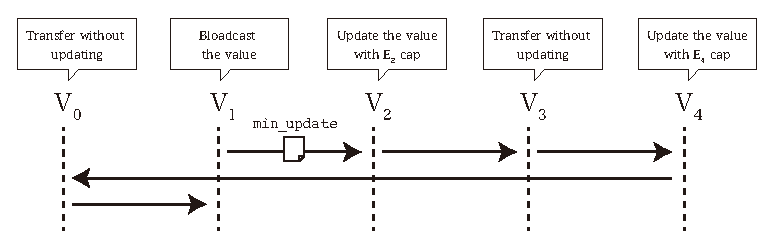
\includegraphics[width=\linewidth]{fig/group_cap_handover}}
	\caption{Group Capacity Calculation Protocol Message Flow}
	\label{fig:group_cap_handover}
\end{figure}

\section{Performance Evaluation}

This section evaluates the latency performance of the proposed GCB method through simulation, where latency is defined as the time elapsed from payment initiation until payment confirmation (regardless of success or failure).

\subsection{Simulation Conditions}
We extended the payment channel network simulator CLoTH~\cite{CONOSCENTI2021100717}, which accurately reproduces Lightning Network HTLCs, by implementing the GCB method.
We used a Lightning Network snapshot from December 17, 2020, containing 6,005 nodes and 60,913 links.
This data was obtained from LND's~\cite{lnd} \texttt{describegraph} command and contains all publicly available information identical to that in the actual network.
Since initial payment channel balances are not published, we set them using uniformly distributed random values.
We performed 5,000 payments with amounts following a normal distribution (mean $\mu = 10,000$ satoshis, variance $\sigma = \mu \times 0.1$) and uniformly distributed random sender and recipient selection.

\subsection{Latency Evaluation}

We compared the GCB method with the conventional Lightning Network probabilistic routing method for varying payment amounts at a time.
The results show that while the conventional method's confirmation delays increase significantly with payment amount, the GCB method's delays increase relatively little.
For large amounts of payments, the conventional method experiences many retries since it does not have information of actual link capacity and judges link availability only by its past failure frequency, thereby prolonging confirmation time.
The GCB method eliminates unnecessary retries by disclosing conservative capacity bounds, enabling immediate pre-transmission determination of infeasible payments and minimizing confirmation delay increases even for large amounts, as demonstrated in Fig.~\ref{fig:pmt_amt_vs_time}.

\begin{figure}[htbp]
	\centerline{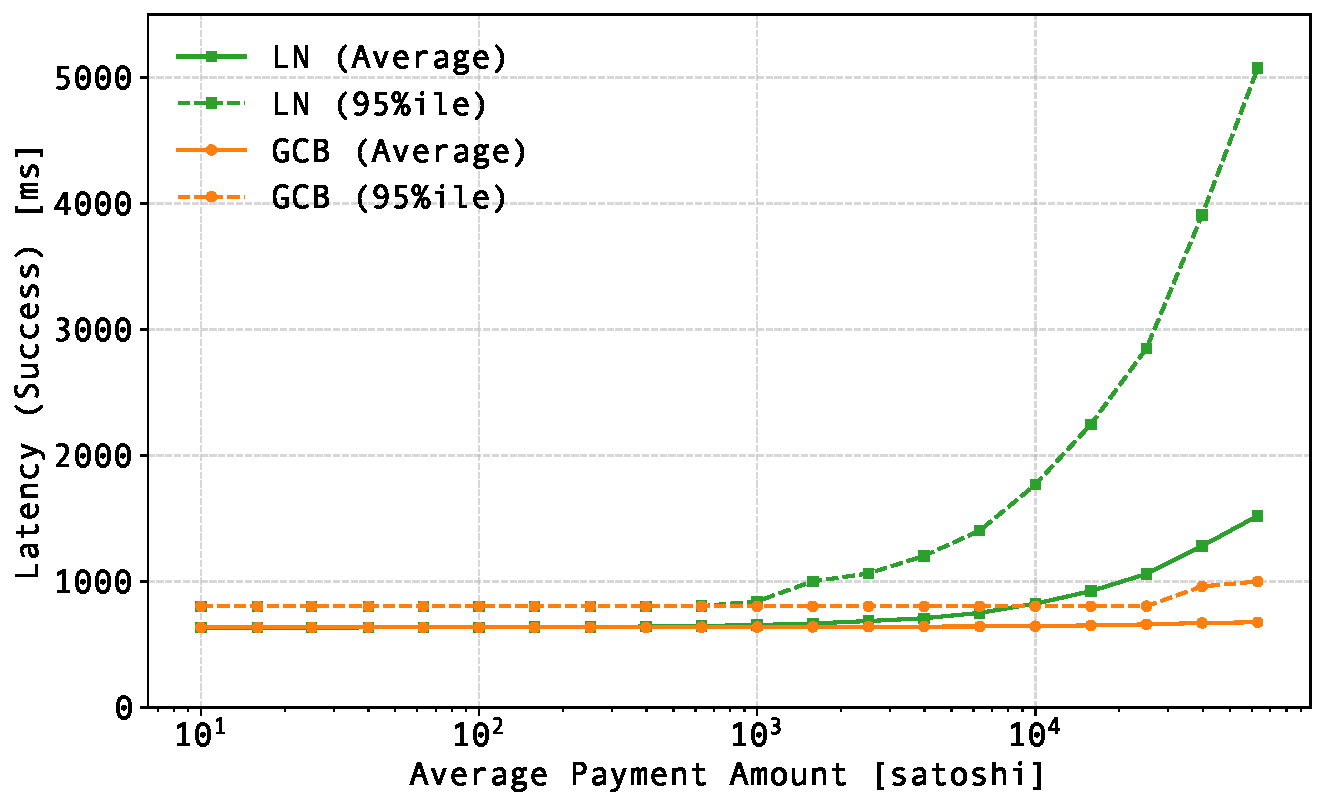
\includegraphics[width=\linewidth]{fig/pmt_amt_vs_time}}
	\caption{Latency of Sending Payment vs Payment Amount for Successful Cases Only}
	\label{fig:pmt_amt_vs_time}
\end{figure}

\begin{thebibliography}{00}
	\bibitem{poon_dryja_2016} J. Poon and T. Dryja, ``The bitcoin lightning network: Scalable off-chain instant payments,'' 2016.
	\bibitem{nakamoto2008bitcoin} S. Nakamoto, ``Bitcoin: A peer-to-peer electronic cash system,'' 2008.
	\bibitem{lnbolt} ``BOLT: Basis of Lightning Technology,'' \url{https://github.com/lightningnetwork/lightning-rfc}.
	\bibitem{lnd} ``Lightning Network Daemon,'' \url{https://github.com/lightningnetwork/lnd}.
	\bibitem{clightning} ``Core Lightning,'' \url{https://github.com/ElementsProject/lightning}.
	\bibitem{eclair} ``Eclair,'' \url{https://github.com/ACINQ/eclair}.
	\bibitem{CONOSCENTI2021100717} M. Conoscenti et al., ``CLoTH: A simulator for HTLC payment networks,'' Future Generation Computer Systems, vol. 118, pp. 1--17, 2021.
\end{thebibliography}

\end{document}
